% !TEX TS-program = XeLaTeX
% use the following command:
% all document files must be coded in UTF-8
\documentclass[spanish]{textolivre}
% build HTML with: make4ht -e build.lua -c textolivre.cfg -x -u article "fn-in,svg,pic-align"

\journalname{Texto Livre}
\thevolume{17}
%\thenumber{1} % old template
\theyear{2024}
\receiveddate{\DTMdisplaydate{2023}{7}{28}{-1}} % YYYY MM DD
\accepteddate{\DTMdisplaydate{2023}{10}{9}{-1}}
\publisheddate{\DTMdisplaydate{2023}{11}{13}{-1}}
\corrauthor{Olga Fernández-Juliá}
\articledoi{10.1590/1983-3652.2024.47493}
%\articleid{NNNN} % if the article ID is not the last 5 numbers of its DOI, provide it using \articleid{} commmand 
% list of available sesscions in the journal: articles, dossier, reports, essays, reviews, interviews, editorial
\articlesessionname{dossier}
\runningauthor{Fernández-Juliá y Gómez-Camacho} 
%\editorname{Leonardo Araújo} % old template
\sectioneditorname{Hugo Heredia Ponce}
\layouteditorname{Thaís Coutinho}

\title{Norma digital y competencia ortográfica de adolescentes en contextos vulnerables: un estudio de casos}
\othertitle{Norma digital e competência ortográfica de adolescentes em contextos vulneráveis: um estudo de casos}
\othertitle{Digital norm and spelling competence of adolescents in vulnerable contexts: a case study}
% if there is a third language title, add here:
%\othertitle{Artikelvorlage zur Einreichung beim Texto Livre Journal}

\author[1]{Olga Fernández-Juliá~\orcid{0000-0002-5126-3666}\thanks{Email: \href{mailto:ofernandez@us.es}{ofernandez@us.es}}}
\author[1]{Alejandro Gómez-Camacho~\orcid{0000-0002-6431-6405}\thanks{Email: \href{mailto:agomez21@us.es}{agomez21@us.es}}}
\affil[1]{Universidad de Sevilla, Departamento de Didáctica de la lengua y la literatura y Filologías Integradas, Sevilla, España.}

\addbibresource{article.bib}
% use biber instead of bibtex
% $ biber article

% used to create dummy text for the template file
\definecolor{dark-gray}{gray}{0.35} % color used to display dummy texts
\usepackage{lipsum}
\SetLipsumParListSurrounders{\colorlet{oldcolor}{.}\color{dark-gray}}{\color{oldcolor}}

% used here only to provide the XeLaTeX and BibTeX logos
\usepackage{hologo}

% if you use multirows in a table, include the multirow package
\usepackage{multirow}

% provides sidewaysfigure environment
\usepackage{rotating}

% CUSTOM EPIGRAPH - BEGIN 
%%% https://tex.stackexchange.com/questions/193178/specific-epigraph-style
\usepackage{epigraph}
\renewcommand\textflush{flushright}
\makeatletter
\newlength\epitextskip
\pretocmd{\@epitext}{\em}{}{}
\apptocmd{\@epitext}{\em}{}{}
\patchcmd{\epigraph}{\@epitext{#1}\\}{\@epitext{#1}\\[\epitextskip]}{}{}
\makeatother
\setlength\epigraphrule{0pt}
\setlength\epitextskip{0.5ex}
\setlength\epigraphwidth{.7\textwidth}
% CUSTOM EPIGRAPH - END

% LANGUAGE - BEGIN
% ARABIC
% for languages that use special fonts, you must provide the typeface that will be used
% \setotherlanguage{arabic}
% \newfontfamily\arabicfont[Script=Arabic]{Amiri}
% \newfontfamily\arabicfontsf[Script=Arabic]{Amiri}
% \newfontfamily\arabicfonttt[Script=Arabic]{Amiri}
%
% in the article, to add arabic text use: \textlang{arabic}{ ... }
%
% RUSSIAN
% for russian text we also need to define fonts with support for Cyrillic script
% \usepackage{fontspec}
% \setotherlanguage{russian}
% \newfontfamily\cyrillicfont{Times New Roman}
% \newfontfamily\cyrillicfontsf{Times New Roman}[Script=Cyrillic]
% \newfontfamily\cyrillicfonttt{Times New Roman}[Script=Cyrillic]
%
% in the text use \begin{russian} ... \end{russian}
% LANGUAGE - END

% EMOJIS - BEGIN
% to use emoticons in your manuscript
% https://stackoverflow.com/questions/190145/how-to-insert-emoticons-in-latex/57076064
% using font Symbola, which has full support
% the font may be downloaded at:
% https://dn-works.com/ufas/
% add to preamble:
\newfontfamily\Symbola{Symbola}
% in the text use:
% {\Symbola }
% EMOJIS - END

% LABEL REFERENCE TO DESCRIPTIVE LIST - BEGIN
% reference itens in a descriptive list using their labels instead of numbers
% insert the code below in the preambule:
%\makeatletter
%\let\orgdescriptionlabel\descriptionlabel
%\renewcommand*{\descriptionlabel}[1]{%
%  \let\orglabel\label
%  \let\label\@gobble
%  \phantomsection
%  \edef\@currentlabel{#1\unskip}%
%  \let\label\orglabel
%  \orgdescriptionlabel{#1}%
%}
%\makeatother
%
% in your document, use as illustraded here:
%\begin{description}
%  \item[first\label{itm1}] this is only an example;
%  % ...  add more items
%\end{description}
% LABEL REFERENCE TO DESCRIPTIVE LIST - END


% add line numbers for submission
%\usepackage{lineno}
%\linenumbers

\begin{document}
\maketitle

\begin{polyabstract}
\begin{abstract}
Este artículo de investigación examina la relación entre la competencia ortográfica y la competencia digital en estudiantes de Educación Secundaria Obligatoria en contextos vulnerables. Se realizó un estudio de casos comparando dos centros de educación secundaria en zonas con necesidad de transformación social con dos centros sin problemas de integración social. La muestra consistió en 126 estudiantes de edades entre 14 y 16 años, seleccionados de manera intencional. Los resultados indican que no hay diferencias significativas en la relación entre ortografía académica y el uso de textismos en la comunicación digital en ambos tipos de centros. Se concluye que la escritura digital no perjudica la ortografía académica de los estudiantes adolescentes, independientemente de su entorno. Sin embargo, el alumnado de centros en zonas con necesidades de transformación social presentan un uso diferenciado de la norma digital: utilizan menos textismos léxicos, semánticos y multimodales, y cometen un número mayor de faltas de ortografía. Estos hallazgos destacan la necesidad de abordar de manera diferenciada la competencia ortográfica y digital en el ámbito educativo para los estudiantes según en contexto en el que vivan y estudien.

\keywords{Textismos \sep WhatsApp \sep Comunicación digital \sep Zonas de necesidad de transformación social \sep Contextos vulnerables}
\end{abstract}

\begin{portuguese}
\begin{abstract}
Este artigo de pesquisa examina a relação entre competência ortográfica e competência digital em estudantes do Ensino Secundário Obrigatório em contextos vulneráveis. Foi realizado um estudo de casos comparando duas escolas secundárias em áreas carentes de transformação social com duas escolas sem problemas de integração social. A amostra consistiu em 126 estudantes com idades entre 14 e 16 anos, selecionados de forma intencional. Os resultados indicam que não há diferenças significativas na relação entre ortografia acadêmica e o uso de textismos na comunicação digital em ambos os tipos de escolas. Conclui-se que a escrita digital não prejudica a ortografia acadêmica dos estudantes adolescentes, independentemente do ambiente em que vivem. No entanto, os alunos das escolas em áreas carentes de transformação social apresentam um uso diferenciado da norma digital: utilizam menos textismos léxicos, semânticos e multimodais, e cometem um número maior de erros ortográficos. Essas descobertas destacam a necessidade de abordar de forma diferenciada a competência ortográfica e digital no contexto educacional para os estudantes, dependendo do contexto em que vivem e estudam.

\keywords{Textismos \sep WhatsApp \sep Comunicação digital \sep Zonas de necessidade de transformação social \sep Contextos vulneráveis}
\end{abstract}
\end{portuguese}

\begin{english}
\begin{abstract}
This research article examines the relationship between spelling competence and digital competence in students of compulsory secondary education in vulnerable settings. A case study was conducted comparing two secondary education centres in areas in need of social transformation with two centres without social integration problems. The sample consisted of 126 students aged 14 to 16 years, intentionally selected. The results indicate that there are no significant differences in the relationship between academic spelling and the use of textisms in digital communication in both types of centres. It is concluded that digital writing does not harm the academic spelling of adolescents, regardless of their environment. However, students in centres in areas with social transformation needs exhibit a differentiated use of the digital norm: They use fewer lexical, semantic, and multimodal textisms and commit a greater number of spelling errors. These findings emphasise the need to address spelling and digital competence differently in the educational context for students, depending on the context in which they live and study.

\keywords{Textisms \sep WhatsApp \sep Digital Communication \sep Areas with social transformation needs \sep Vulnerable contexts}
\end{abstract}
\end{english}

% if there is another abstract, insert it here using the same scheme
\end{polyabstract}

\section{Introducción}

\subsection{Comunicación digital y textismos}

WhatsApp ha alcanzado una relevancia extraordinaria en España, convirtiéndose en una herramienta esencial para la comunicación diaria de millones de personas en el país \cite[p. 101]{vazquez-cano_alisis_2015}. Esta popular aplicación de mensajería instantánea ha revolucionado la forma en que los españoles se mantienen conectados; presenta grandes ventajas como la facilidad para enviar mensajes en distinto formato (texto, audio, vídeos...); la posibilidad de responder de manera casi inmediata y su bajo coste \cite{suarez_lantaron_whatsapp:_2018}. También permite realizar llamadas de voz y vídeo \cite{scribano_miradas_nodate}; compartir imágenes y documentos, y en su última actualización, incluso crear encuestas grupales de manera rápida y sencilla. Gracias a su interfaz intuitiva y la posibilidad de crear grupos de chat, WhatsApp facilita a diario la organización de eventos, la coordinación en el trabajo y el contacto con familiares y amigos. Su omnipresencia en los teléfonos móviles de los españoles ha hecho de WhatsApp una herramienta indispensable para mantenerse informado y en contacto con el entorno social y laboral en todo momento \cite{fondevila-gascon_usos_2019}.

Durante el último año, se evidenció que aproximadamente el 94\% de los ciudadanos españoles que hacen uso habitual de internet, utilizaron la plataforma de mensajería instantánea WhatsApp para intercambiar mensajes \cite{comision_nacional_de_los_mercados_y_la_competencia_ocho_nodate}. Cabe destacar que un 65\% afirmó que utilizaba WhatsApp en múltiples ocasiones diarias, mientras que un 30\% manifestó hacerlo una vez al día \cite{statista_distribucion_nodate}. Estos datos reflejan la preeminencia y la frecuencia de uso de WhatsApp como herramienta de comunicación en la sociedad española en la actualidad \cite{molina_garcia_hablamos?_2020}. 

Inevitablemente el uso cotidiano de la aplicación WhatsApp ha influido en la aparición de normas lingüísticas distintas a las establecidas por la Real Academia de la Lengua Española en personas de diversas franjas de edad, en especial en lo que se refiere a la norma de escritura en géneros textuales propios de la comunicación digital \cite{gomez_camacho_norma_2017}. La incidencia de este lenguaje desvinculado de la norma ortográfica ha sido objeto de análisis desde la proliferación de los SMS, donde inicialmente se acortaban palabras debido a la limitación en el número de caracteres en los mensajes enviados, que primaba la máxima información en mensajes breves \cite[p. 358]{forbes_textisms:_2019}; \cite[p. 3]{jacquet_contextual_2021}.

El lenguaje propio de la comunicación mediada por ordenador (Computer-Mediated Communication, CMC) ha sido identificado y denominado con diversos términos, como "Digitalk" \cite[p. 67]{chalak_linguistic_2017}, "textspeak" o "textese" \cite[p. 583]{verheijen_effects_2013} o “norma digital” \cite[p. 61]{gomez-camacho_youth_2023b}. Este "digitalk" o "textese" se caracteriza principalmente por el uso de textismos \cite[p. 7]{burrell_playful_2022}, que consisten en discrepancias intencionadas en la ortografía de palabras y el empleo de abreviaturas en los mensajes de texto \cite{bernicot2014skilled}, y que en ocasiones se utilizan también para transmitir información no verbal en la comunicación textual \cite{adams2023examining}.


\subsection{La relación entre el uso de textismos y la ortografía académica}

Desde los inicios del uso masivo de SMS, se ha observado un creciente número de jóvenes que adoptan un nuevo tipo de lenguaje que prima la brevedad y prescinde de las normas ortográficas y gramaticales convencionales \cite[p. 583]{verheijen_effects_2013}, lo que ha generado inquietud en cuanto a su impacto en la comunicación y en el lenguaje en general \cite[p. 251]{drouin_texting_2014}. Esta preocupación se extiende también al ámbito educativo, donde tanto profesores como padres temen que los alumnos o hijos puedan abandonar las normas del lenguaje estándar al emplear la comunicación digital con tanta frecuencia \cite[p. 16]{totanes_textese_2019}, \cite[p. 112]{verheijen_orthographic_2018}. El análisis de estos patrones lingüísticos en el entorno digital es esencial para una mejor comprensión de los cambios en la comunicación y su impacto en la sociedad actual \cite{adams2023examining}.

Son muchas las publicaciones que en la última década han tratado llegar a alguna conclusión sobre de qué manera puede afectar el uso de textismos a las habilidades de alfabetización \cite{de_jonge_textmessage_2012,drouin_college_2011,grace_undergraduates_2014,ouellette_generation_2016,plester_exploring_2009,van_dijk_influence_2016,wood_longitudinal_2011a}. Por otro lado, existe una serie de artículos que se han centrado en comprobar la relación existente entre el uso de textismos y la lectura \cite{coe_txtn_2011}, la escritura tanto formal como informal \cite{rosen_relationship_2010,torrado_cespon_uso_2015} y, especialmente, la ortografía \cite{bernicot2014skilled,bushnell_text-messaging_2011,gomez_camacho_norma_2017,lanchantin_good_2014,powell_does_2011,wood_effect_2011b}. Los resultados no llegan a conclusiones claras sobre esta relación, probablemente porque se han llevado a cabo con muestras muy diversas desde niños entre 10 y 13 años \cite{van_dijk_influence_2016} hasta adultos, sobre todo jóvenes universitarios \cite{drouin_texting_2014,grace_text_2015,hunt-gomez_textisms_2020,kemp_university_2017,lyddy_analysis_2014}, entre otros factores. 

En consecuencia, no existe un consenso a la hora de responder a la pregunta de en qué manera podrían afectar los textismos a la alfabetización, lo que podría deberse, además de a la diferencia de edades en las muestras, a las grandes discrepancias existentes en las metodologías y a los diversos idiomas analizados \cite{fernandez_julia_textisms_2023,verheijen_effects_2013}.

En el caso de la lengua española, los estudios que se han realizado coinciden en que el uso de textismos no solo no perjudica a la competencia ortográfica del alumnado, sino que la tendencia es a relacionar el uso de textismos con una correcta ortografía académica \cite{gomez-camacho_youth_2023b,gomez_camacho_norma_2017}.

\subsection{La comunicación digital y las faltas de ortografía en los contextos vulnerables}

Pese a que se han llevado a cabo múltiples investigaciones sobre el impacto del uso de textismos en la alfabetización de niños, adolescentes y adultos, estos estudios se han realizado de manera global, sin considerar las distintas características de cada grupo investigado \cite{gomez-camacho_ke_2023a,parrella_measuring_2021,verheijen_relationships_2020}. La bibliografía se ha centrado en el análisis de la influencia del contexto socioeconómico en el rendimiento académico del alumnado \cite{escarbajal_frutos_rendimiento_2019,tique-gutierrez_contexto_2018}. 

En España, se han regulado legislativamente las actuaciones educativas en las zonas denominadas como “Zonas con Necesidades de Transformación Social” (ZNTS) y esta preocupación ha sido un aspecto recurrente y de suma relevancia en todas las reformas legislativas implementadas a lo largo de distintos periodos \cite{arredondo2018zonas}, ya que la infancia es un colectivo especialmente vulnerable \cite[p. 91]{martin_hierro_aprendizaje_2020}.

Como afirman \textcite[p. 181]{gomez-jarabo_vulnerables_2023}, el término de vulnerabilidad aplicado a la educación se manifiesta en aquellas personas que sufren dificultades en su trayectoria escolar, ya sean de acceso al sistema educativo, de dificultades a la hora de continuar con sus estudios o en los resultados académicos que obtienen. Ninguna investigación se ha ocupado hasta ahora de la relación entre textismos y faltas en el alumnado escolarizado en contextos vulnerables.

El presente estudio parte de la hipótesis de que el uso de textismos y su relación con la ortografía académica varía entre adolescentes que se encuentran en contextos vulnerables en comparación con aquellos educados en entornos no vulnerables. Al considerar estas distinciones en el análisis, se busca profundizar en las posibles disparidades en la relación entre el uso de textismos y la ortografía académica en diferentes grupos poblacionales.

Con el objetivo de realizar una comparación adecuada, se ha decidido seleccionar como contextos vulnerables aquellos identificados por la administración educativa como "Zonas con Necesidades de Transformación Social" (ZNTS). Este concepto surgió gracias a la administración de la Junta de Andalucía en los primeros años de la década de los ochenta del siglo pasado. Su objetivo principal era intervenir en aquellos sectores urbanos caracterizados por la concentración de situaciones de vulnerabilidad y exclusión social \cite[p. 27]{munoz-garcia2023}. Según la definición de la \textcite{junta_de_andalucia_zonas_nodate}, estas áreas se caracterizan por congregar situaciones estructurales de pobreza grave y marginación social, evidenciando problemas en diversos aspectos como vivienda, infraestructura, servicios públicos, absentismo y fracaso escolar, desempleo, deficiencias higiénicas-sanitarias, y fenómenos de desintegración social. 

Este trabajo pretende responder a las siguientes preguntas de investigación:

\begin{itemize}
    \item P.I.1. ¿Se utiliza la misma norma digital en aplicaciones de mensajería instantánea por el alumnado de centros ubicados en Zonas con Necesidades de Transformación Social (ZNTS) y el alumnado de centros en zonas sin Necesidades de Transformación Social (ZSNTS)? 
    \item P.I.2. ¿Influye de forma diferenciada el uso de textismos en la comunicación digital en la competencia ortográfica académica de alumnado de centros ZNTS y de centros ZSNTS? 
\end{itemize}


\section{Método}

En esta investigación, se ha optado por el enfoque de estudio de casos, un método de investigación que posibilita el entendimiento de lo peculiar, lo individual y lo singular, enfocándose en lo que se puede extraer como aprendizaje de cada situación específica \cite{Stake1995}. Este enfoque permite además una comprensión profunda de una realidad ya sea de índole social o educativa \cite[p. 302]{Bisquerra}. Para responder a las preguntas de investigación, se ha empleado una metodología cuantitativa, específicamente un diseño descriptivo. Esta combinación de enfoques nos ha proporcionado una visión completa y detallada del fenómeno estudiado, permitiéndonos obtener conclusiones sólidas y fundamentadas \cite{gomez-camacho_ke_2023a}.


\subsection{Muestra}

Siguiendo el modelo de \textcite{gomez-camacho_youth_2023b} para la lengua española, esta investigación se llevó a cabo utilizando un método de muestreo no probabilístico por conveniencia. La muestra consistió en un total de 126 alumnos, con edades comprendidas entre los 14 y los 16 años, pertenecientes a los cursos de 3º y 4º de Educación Secundaria Obligatoria, los dos últimos cursos de enseñanza obligatoria en España. El 54,8\% de los participantes correspondían a alumnos del 3º curso, mientras que el 45,2\% restante pertenecían al 4º curso de Educación Secundaria Obligatoria.

De los 126 alumnos, 39 de ellos asistían a centros ubicados en Zonas con Necesidades de Transformación Social (ZNTS) y provenían de la localidad de Sevilla, específicamente del barrio de Torreblanca y también de la localidad de Sanlúcar de Barrameda, en Cádiz. Por otro lado, los 87 alumnos restantes provenían de centros ubicados en Zonas sin Necesidades de Transformación Social (ZSNTS) y procedían de dos centros diferentes: uno en la ciudad de Dos Hermanas (Sevilla), y otro en la localidad de Jaén.

En términos de género, el 47,6\% de la muestra eran mujeres, mientras que el 31\% eran hombres. El 21,6\% restante no proporcionó esta información. La muestra ofrece una base sólida para el análisis comparativo entre los estudiantes de centros ZNTS y ZSNTS en relación con el uso de textismos en la comunicación digital y las faltas de ortografía en la escritura académica.



\subsection{Instrumento}

En esta investigación se ha utilizado el instrumento validado en el estudio de \textcite{gomez-camacho_youth_2023b}. Se utilizó una hoja de registro donde se anotaron los textismos por repeticiones enfáticas, omisiones, grafemas no normativos, textismos léxicos y elementos multimodales.

Para facilitar el análisis los textismos también se agruparon en textismos del plano léxico-semántico, textismos dialectales, textismos por repetición y textismos por acortamiento. 


\subsection{Recogida de datos}

El análisis de la comunicación digital de esta investigación se ha efectuado sobre los mensajes reales que los adolescentes envían a través de sus teléfonos inteligentes mediante la aplicación de WhatsApp. Para ello, se les pidió que copiaran y pegaran en un documento entre 10 y 20 intervenciones de WhatsApp que fueran representativas de su manera de escribir por esta aplicación y se les insistió en que en ningún caso debían modificar palabras o letras, ni hacer ningún tipo de corrección. Además, se les indicó que debían eliminar cualquier dato de carácter privado que apareciese, así como referencias a nombres propios. 

Los textismos fueron identificados y codificados manualmente siguiendo el modelo de \textcite[p. 119]{verheijen_orthographic_2018} en una investigación similar.

Por otra parte, para conocer la competencia ortográfica en la escritura académica de los adolescentes, se les pidió que escaneasen con sus teléfonos inteligentes una o dos páginas manuscritas de sus apuntes o actividades de clase con los mismos requerimientos que en los textos de la comunicación digital.  



\subsection{Análisis de datos}

Para analizar estadísticamente los datos se ha utilizado el software IBM SPSS en su versión 27. Se han realizado análisis descriptivos y de correlación bivariada.


\section{Resultados}

El corpus resultante del análisis está compuesto por un total 12297 palabras, siendo la media de 97,6 unidades léxicas, compuestas tanto por palabras como por otras unidades de comunicación como stickers, emoticonos o GIF por cada estudiante (SD=38,79). El número máximo de palabras por alumno ha sido de 218 y el mínimo de 22. El corpus se caracteriza por una media de 20,09 intervenciones en las que se utilizaron una media de 32,06 textismos por alumno (SD=16,24).

Por otra parte, en los textos académicos presentados por el alumnado se han examinado un total de 22802 palabras. La media de palabras de estos textos ha sido de 183,89 (SD=77,22) siendo el valor mínimo 38 y el valor máximo 465.  La media de faltas en los textos académicos del corpus fue de 5,22 (SD=5,474).

En primer lugar, se realizó un análisis estadístico descriptivo de los textismos y las faltas en ambos tipos de centros (\Cref{tbl1}).

\begin{table}[htbp]
\caption{Análisis del uso de textismos.}
\label{tbl1}
\centering
%\begin{tabular}{p{5.5cm} p{1.0cm} p{1.0cm} p{3.5cm}}
\begin{tabular}{llll}
\toprule
 & \multicolumn{1}{p{1.0cm}}{Centros ZNTS} & \multicolumn{1}{p{1.0cm}}{Centros ZSNTS} & Ejemplos del corpus \\ \midrule
Nº total de textismos del texto de WhatsApp & 33,51 & 31,45 & \\ 
Unión intencionada de palabras & 2,77 & 2,84 & “Digual”, “nidea” “nose” \\
Acortamiento de palabras  & 11,44 & 10,39 & “Mñna”, “llgndo” “q” \\
Repetición de marcas de cierre  & ,44 & ,53 & “No te quieren??” \\
Omisión de signos de puntuación & 2,74 & 3,54 & “A donde”, “ya qieres qeda?” \\
Omisión tildes & 4,69 & 4,89 & “si”, “super”, “tu” \\
Palabras en inglés & ,97 & 1,07 & “anyways”, “thanks” “omg” \\
Elementos multimodales  & ,38 & 1,22 & {\fontspec{Symbola}\symbol{"1F60E}\symbol{"2764}\symbol{"1F600}} \\
Nº total de faltas  & 5,9 & 4,91 & \\
\bottomrule
\end{tabular}
\source{Elaboración propia.}
\end{table}

%Inserir emojis na penúltima linha da tabela 1


En el contexto de la primera pregunta de investigación, no se observan grandes diferencias entre ambos tipos de centros con la excepción del uso de elementos multimodales que triplica su uso en los centros ZSNTS. Por el contrario, el número total de faltas y el número total de textismos es superior en los centros ZNTS, lo que ofrece una diferencia en ambos tipos de centros para responder a la segunda pregunta de investigación. 

Con el objetivo de facilitar el análisis y la comparación de resultados con estudios precedentes, también se recogieron los valores medios de los textismos dialectales \cite{gomez-camacho_ke_2023a}, textismos del plano léxico-semántico \cite{gomez-camacho_youth_2023b} y textismos por repetición \cite{verheijen_orthographic_2018} y acortamiento \cite{adams2023examining} (\Cref{fig1}).

\begin{figure}[htbp]
\centering
\begin{minipage}{.9\textwidth}
 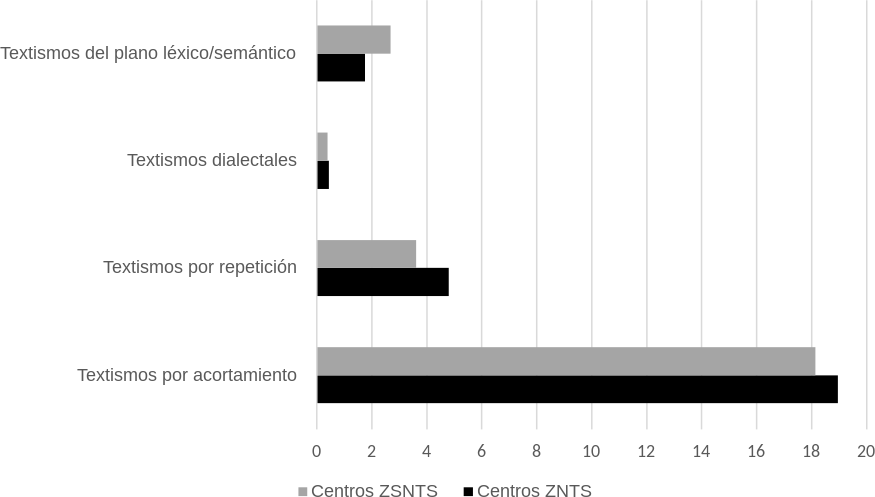
\includegraphics[width=\textwidth]{Fig1.png}
 \caption{Uso de los distintos tipos de textismos en centros ZSNTS y ZNTS}
 \label{fig1}
 \source{Elaboración propia.}
\end{minipage}
\end{figure}

Los textismos más frecuentes en ambos tipos de centros son los textismos por acortamiento, con una media de 18,97 en los centros ZNTS y de 18,16 en los centros ZSNTS. Los textismos por repetición presentan una media de uso de 4,82 en los centros ZNTS y de 3,62 en los centros ZSNTS. Los textismos del plano léxico-semántico son utilizados una media de 1,77 veces por alumno en los en centros ZNTS y de 2,69 en centros ZSNTS.

Por último, los textismos menos utilizados en esta clasificación son los textismos dialectales, con una media de 0,46 en los centros ZNTS y de 0,40 en los centros ZSNTS. En consecuencia, los centros ZNTS utilizan más textismos en la comunicación digital excepto en el plano léxico-semántico.

En segundo lugar, se hizo un análisis correlacional entre los textismos de la \Cref{tbl1}, el número total de textismos y el número total de faltas de ortografía en los textos académicos (\Cref{tbl2}). 

\begin{table}[h!]
\centering
\begin{small}
\caption{Correlaciones entre los distintos tipos de textismos y las faltas de ortografía.}
\label{tbl2}
\footnotesize
\begin{tabular}{>{\raggedright}p{1.5cm}lllllllll}
\toprule
 &  & 
 \multicolumn{1}{>{\raggedright}p{1.0cm}}{Unión intencionada de palabras} & 
 \multicolumn{1}{>{\raggedright}p{1.0cm}}{Acorta\-mien\-to de palabras} & 
 \multicolumn{1}{>{\raggedright}p{1.0cm}}{Omisión tildes} & 
 \multicolumn{1}{>{\raggedright}p{1.0cm}}{Omisión signos puntuación} & 
 \multicolumn{1}{>{\raggedright}p{1.0cm}}{Palabras en inglés} & 
 \multicolumn{1}{>{\raggedright}p{1.0cm}}{Elementos multimodales} & 
 \multicolumn{1}{>{\raggedright}p{1.0cm}}{Grafemas no normativos} & 
 \multicolumn{1}{>{\raggedright}p{1.0cm}}{Nº total de faltas} \\ 
\midrule
Nº total de textismos & ZNTS & ,737** & ,726** & ,141 & -,147 & ,170 & -,306 & ,339* & ,219 \\
& ZSNTS & ,811** & ,876** & ,224* & .086 & ,069 & ,119 & ,431** & -,043 \\
%\midrule
Unión intencionada de palabras; & ZNTS  & & ,483** & ,064 & -,194 & ,037 & -,195 & ,188 & ,003 \\
& ZSNTS & & ,718** & ,116 & ,359 & -,017 & ,080 & ,366** & ,053 \\
%\midrule
Acortamiento de palabras & ZNTS & & & -,176 & -,227 & -,111 & -,274 & ,234 & ,155 \\
& ZSNTS & & & ,090 & .074 & -,159 & -,131 & ,347** & -,074 \\
%\midrule
Omisión tildes & ZNTS & & & & ,273 & -,082 & -,150 & ,032 & ,220 \\
& ZSNTS & & & & ,099 & -,191 & -,122 & -,074 & ,306** \\
%\midrule
Omisión signos de puntuación & ZNTS & & & & & -,149 & -,255* & -,170 & ,273 \\
& ZSNTS & & & & & -,147 & -,229* & -,239 & -,119 \\
%\midrule
\multirow{2}{*}{} Palabras en inglés & ZNTS & & & & & & ,123 &
,095 & -,054 \\
& ZSNTS & & & & & & ,313** & -,047 & -,165 \\
%\midrule
Elementos multimodales & ZNTS & & & & & & & -,146 & 
-,031 \\
& ZSNTS & & & & & & & ,227* & -,083 \\
%\midrule
Grafemas no normativos & ZNTS & & & & & & & & ,1 \\
& ZSNTS & & & & & & & & -,024 \\
\bottomrule
\end{tabular}
\source{Elaboración propia.}
\end{small}
\end{table}



Las correlaciones muestran diferencias interesantes en los dos grupos analizados que sirven para responder a la primera pregunta de investigación sobre el uso de la norma digital en ambos grupos.

En los centros ZNTS la correlación entre los diferentes tipos de textismos, así como con el número total de textismos tiende a ser más baja. Especialmente interesante es la correlación significativa en el nivel 0,01 y directa entre los textismos de unión intencionada de palabras y de acortamiento de palabras con un valor de $r=,483$, frente al valor de $r=,718$ en los centros ubicados en ZSNTS.

Las diferencias más notables desde el punto de vista correlacional entre los dos grupos estudiados se establecen en el contexto del uso de elementos multimodales en la comunicación a través de aplicaciones de mensajería instantánea.  Los textismos de palabras en inglés establecen una correlación de $r=,313$ en ZSNTS frente a $r=,123$ en centros ZNTS. En otras palabras, la norma digital empleada en centros ZSNTS se diferencia por la relación entre elementos multimodales y el uso de palabras en inglés frente a los centros ZNTS.  

Sin embargo, no encontramos diferencias en la norma digital utilizada desde el punto de vista correlacional en los textismos por omisión de signos de puntuación, que presentan una correlación significativa en el nivel 0,05 con textismos de elementos multimodales en los centros ubicados en centros ZNTS con un valor de $r=-,255$ y en los centros ZSNTS con un valor de $r=-,229$.

El análisis correlacional también ofrece datos para responder a la segunda pregunta de investigación sobre las consecuencias educativas del uso de textismos en los dos grupos. 

Los resultados no muestran una correlación significativa entre faltas y textismos en ninguno de los grupos analizados. Considerando el número total de faltas y el número total de textismos, la correlación entre ambos es positiva $r=,219$ en centros ZNTS y negativa $r=-,043$ en centros ZSNTS. Aunque no son correlaciones significativas estadísticamente, la tendencia indica que solo en centros ZSNTS el uso de textismos se asociaría a una buena ortografía académica. 

El ejemplo más ilustrativo lo encontramos en el uso de los grafemas no normativos, que son los que por su naturaleza pueden identificarse con mayor facilidad con faltas de ortografía. La correlación de estos textismos con el número total de faltas es de ,1 en centros ZNTS y de -,024 en ZSNTS. 

Esta tendencia no se confirma en el caso de los textismos por omisión de tildes en ninguno de los dos grupos, lo que sugiere que los textismos y las faltas relacionadas con las tildes deberían ser considerados de forma independiente. 



\section{Discusiones y conclusión}

El objetivo principal del presente estudio es el análisis de la relación entre norma digital en WhatsApp y la competencia ortográfica de los adolescentes andaluces tanto en contextos vulnerables como en contextos no vulnerables, así como la relación que podría establecerse con su ortografía en la escritura académica. 

En cuanto a la primera pregunta de investigación, podemos afirmar que la norma digital que utilizan los adolescentes andaluces de entre 14 y 16 años es muy parecida, independientemente de las características socioeconómicas de la zona en la que están localizados sus centros educativos. En consecuencia, nuestros datos confirman que el uso de textismos se ha convertido en un fenómeno universal para los jóvenes y todos se comunican utilizando estos nuevos mecanismos. La multimodalidad en los mensajes enviados a través de aplicaciones de mensajería instantánea es la principal diferencia en la norma digital en los dos tipos de centros analizados. Como se describió en resultados, el uso de elementos multimodales caracteriza la comunicación digital en los centros ubicados en ZSNTS, mientras que es mucho menos frecuente en centros en ZNTS. Una conclusión de este estudio es que el alumnado de centros ZSNTS comete menos errores y utiliza más textismos del plano léxico-semántico y multimodal.

Más complejo resulta responder a la segunda pregunta de investigación que indagaba sobre la relación que existe entre el uso de textismos y las faltas de ortografía que se cometen en los textos académicos en ambos contextos educativos. Nuestros datos muestran una tendencia no significativa desde el punto de vista estadístico, pero muy interesante desde el punto de vista educativo en la que los textismos y las faltas de ortografía correlacionan de forma negativa en los centros situados en ZSNTS, mientras que en los centros ubicados en las llamadas ZNTS la tendencia es una correlación positiva. Esto supone que solo los resultados de los centros ubicados en ZSNTS confirman las conclusiones de estudios precedentes en el sentido de que en ningún caso se puede sugerir que el uso de textismos perjudique la ortografía o la alfabetización académica del alumnado adolescente \cite{bernicot2014skilled,ouellette_generation_2016,van_dijk_influence_2016,wood_exploring_2014} o que asocian el uso de textismos con una buena ortografía académica \cite{de_jonge_textmessage_2012}.

El estudio de \textcite{bernicot2014skilled} ya advertía para la lengua francesa de un comportamiento diferenciado de los textismos que alteraban la relación de grafemas y fonemas de la ortografía culta. Nuestros resultados confirman que el uso de grafemas no normativos como textismos pueden asociarse con faltas de ortografía, pero solo en los centros ZNTS. En otras palabras, no se puede afirmar con carácter general que el uso de textismos no perjudique a la ortografía académica de los adolescentes; este axioma debe ser matizado en función del tipo de textismo, y del nivel socioeconómico y cultural de ese alumnado.

Por otro lado, en cuanto a la relación entre el uso de textismos de omisión de tildes y signos auxiliares en la escritura digital con las faltas de ortografía en la escritura académica, encontramos un comportamiento diferente al mencionado con anterioridad. En este caso, la omisión de tildes en los mensajes de texto correlaciona positivamente con las faltas de ortografía en los textos académicos en ambos tipos de centros, ZSNTS y ZNTS. Esta conclusión coincide con la del estudio de \textcite{gomez-camacho_youth_2023b} quienes resaltan la importancia de tratar a este tipo de textismo de manera diferenciada con el resto debido a su comprobado impacto negativo en la escritura académica.

También influyen de una forma diferenciada en la competencia ortográfica en los centros ZTNS y ZSNTS los elementos multimodales. En concreto, se asocian a una buena ortografía y al uso de palabras en inglés solo en los centros ZSNTS. En consecuencia, las conclusiones como la de \textcite{gomez-camacho_textisms_2018} solo se confirman en este tipo de centros, pero no en los centros ZNTS. En nuestra opinión, la utilización de la norma digital y la multimodalidad como recurso para la alfabetización académica del alumnado adolescente debe hacerse de una forma diferenciada en los centros ZNTS, y no sirven las conclusiones generales aplicadas al alumnado adolescente sin considerar su entorno socioeconómico. 

En conclusión, nuestros datos confirman que es necesario adoptar un enfoque diferenciado al abordar la relación entre norma digital y norma académica en los centros ZNTS, reconociendo que el impacto de la comunicación digital no puede ser evaluado de manera holística, sino que debe ser comprendido en función de las realidades específicas que influyen en su manifestación.

Limitaciones del estudio:
El presente estudio se encuentra sujeto a ciertas limitaciones que es importante mencionar. En primer lugar, el número de participantes, si bien proporciona información valiosa, debería ser ampliado en estudios posteriores para alcanzar resultados válidos en el ámbito panhispánico más allá de los hablantes dialectales andaluces. 

Adicionalmente, es relevante señalar que el diseño de tipo descriptivo empleado en este estudio solo permite obtener una instantánea de los datos recopilados en un momento específico. Un estudio longitudinal e internacional permitiría describir la norma digital y sus variedades en contextos diatópicos y diacrónicos. 

Estas limitaciones ofrecen una oportunidad para identificar áreas de mejora en futuras investigaciones, y para proponer enfoques que permitan una comprensión más completa y profunda del fenómeno estudiado.

\section{Financiación}

“Este estudio forma parte de la tesis doctoral titulada "Textismos y norma digital del alumnado adolescente" de Olga Fernández-Juliá, bajo la dirección de Alejandro Gómez-Camacho. Este artículo también está vinculado al proyecto “La escritura digital del alumnado adolescente en Andalucía. La mensajería instantánea y sus implicaciones educativas” (US-1380916) de la Universidad de Sevilla cofinanciado por el Programa Operativo FEDER 2014-2020 de la Unión Europea y por la Consejería de Transformación Económica, Industria, Conocimiento y Universidades de la Junta de Andalucía (España).

\printbibliography\label{sec-bib}
% if the text is not in Portuguese, it might be necessary to use the code below instead to print the correct ABNT abbreviations [s.n.], [s.l.]
%\begin{portuguese}
%\printbibliography[title={Bibliography}]
%\end{portuguese}


%full list: conceptualization,datacuration,formalanalysis,funding,investigation,methodology,projadm,resources,software,supervision,validation,visualization,writing,review
\begin{contributors}[sec-contributors]
\authorcontribution{Olga Fernández-Juliá}[conceptualization,investigation,methodology,writing,review]
\authorcontribution{Alejandro Gómez-Camacho}[conceptualization,methodology,writing,review]
\end{contributors}




\end{document}

